\documentclass{article}
\usepackage[margin=.5in]{geometry}
\usepackage{graphicx, dblfloatfix}
\usepackage{amsmath, amssymb, amsfonts, mathrsfs, mathtools}
\usepackage[english]{babel}
\usepackage[autostyle, english = american]{csquotes}
\usepackage[normalem]{ulem}
\usepackage[title,titletoc,toc]{appendix}
\usepackage{pgfplotstable}
\usepackage{array, booktabs, colortbl}
\MakeOuterQuote{"}

\pgfplotsset{compat=1.12}


\newcommand{\redchi}{$\tilde{\chi}^2\,$}
\DeclareMathOperator{\erf}{erf}
\DeclareMathOperator{\cov}{cov}
\DeclarePairedDelimiter\abs{\lvert}{\rvert}%
\DeclarePairedDelimiter{\parens}{\lparen}{\rparen}

\title{Optical Pumping}
\author{Aman LaChapelle}

\begin{document}
\raggedright
\maketitle

\begin{abstract}
  We investigate the effects of an applied external field on Rubidium-87 atoms, known as Zeeman splitting.  We will further investigate the process known as optical pumping, which is used to excite electrons from the $^2S_{1/2},\, f = 2$ state to the $^2P_{1/2},\, f = 2$ state with the goal of creating a fully pumped state, characterized by a majority of electrons in the $^2S_{1/2},\, f = 2,\, m_f = 2$ state.  Using this pumped state and the requrements surrounding its creation, we will further investigate stimulated emission of photons as well as Larmor Precession, which occurs under another special set of circumstances.
\end{abstract}

\tableofcontents
\newpage

\section{Introduction}%%%%%%%%%%%%%%%%%%%%%%%%%%%%%%%%%%%%%%%%%%%%%%%%%%%%%%%%%
  Here we investigate the effects of Zeeman splitting on Rubidium-87 atoms.  More precisely, we investigate the process that is undertaken in order to 'pump' the atoms into an excited state.  There are many uses for such a process, there are certain times when it is simply advantageous to have a macroscopic number of atoms in a single, well-defined state which this process can achieve.  Another possible application is to construct a 3-level system (as opposed to the 2-level system we encounter here) and use that to achieve true population inversion in order to create a laser.

  Returning to the task at hand, we investigate, specifically, properties of the $^2S_{1/2}, f = 2, m_f = 2$ state.  Due to thermal fluctuations and the fact that this particular state is an excited state of Rb-87, it is highly unlikely that a macroscopic portion of the atoms will be in that particular state at any given time, so we must find a way to put them there.

  While there exist methods to perform this action - that is, pump Rb-87 into a given state, we perform checks to be certain that they are doing what we expect them to do.  We also take measurements to ensure that we aren't seeing a figment of some other effect and that we are in fact seeing optical pumping of the Rb-87 atoms into the state we have selected.
\section{Theory}%%%%%%%%%%%%%%%%%%%%%%%%%%%%%%%%%%%%%%%%%%%%%%%%%%%%%%%%%%%%%%%
  \subsection{Zeeman Effect}
    The Zeeman effect occurs because of an applied magnetic field onto an atom.  It causes a coupling between the atom's magnetic dipole and the external field, which causes an energy splitting.  The energy perturbation is simple, given by
    \begin{equation*}
      \Delta = -\vec{\mu} \cdot \vec{B}.
    \end{equation*}
    This can be simplified, or expanded into a form that depends more obviously on the quantum numbers of the atom like so
    \begin{gather*}
      \Delta = g_f \mu_B \abs{\vec{B}} m_f \\
      \mu_B = \frac{e \hbar}{2m_e} \\
      g_f = g_j\frac{f(f+1) + j(j+1) - i(i+1)}{2f(f+1)} \\
      g_j = 1 + \frac{j(j+1) + s(s+1) - \ell(\ell+1)}{2j(j+1)}
    \end{gather*}
    It should be noted that each of these statements depend on the state that the atom is in, but here we take a single value of $g_f$ (and thus $g_j$), and so we can use the following approximation to calculate the energy level separation
    \begin{equation}
      \delta = (5.79 \times 10^{-9} \, \frac{eV}{G}) g_f \Delta m_f \abs{\vec{B}}.
    \end{equation}

  \subsection{Thermal Noise, Boltzmann and Bose-Einstein Statistics}
    Because there is a certain amount of noise in the energy spectrum simply due to the ambient energy in the room, we must find some way to account for how many atoms are in any given state at any certain time.  Luckily Bose and Einstein built on the foundation of Boltzmann and delivered to us Bose-Einstein statistics to understand the energy distributions of the atoms due to thermal noise.  We can begin from the partition function and write (assuming the atoms do not interact and are indistinguishable)
    \begin{gather*}
      \mathcal{Z} = \sum_j{n_{\epsilon}e^{\frac{\epsilon_j}{k_B T}}} \\
      \text{we introduce}\,\, \beta = \frac{1}{k_B T} \,\, \text{and write}\\
      \mathcal{Z} = \frac{1}{1 - e^{-\beta (\epsilon_j - \mu)}}
    \end{gather*}
    where $\mu$ is the chemical potential attributed to that particular site/atom.  We can, from this, derive the average number of atoms in each state as
    \begin{equation*}
      \bar{N} = \frac{1}{e^{\beta(\epsilon - \mu)} - 1}
    \end{equation*}
    We can find this number, $\bar{N}$ for each of the energy levels in question and describe the system in this way - creating a map of the number of particles in each state versus the energy of each state.  Because of this, we can calculate the ratio of occupations between the $^2S_{1/2}, f = 2, m_f = \pm 2$ states.  In this example, the $m_f = -2$ state is lower energy.
    \begin{gather*}
      \frac{N_{m_f = 2}}{N_{m_f = -2}} = \frac{N_1}{N_2} = \frac{e^{\beta \Delta_{m_f = 2}} - 1}{e^{\beta \Delta_{m_f = -2}} - 1} \\
      \frac{N_1}{N_2}  = \frac{e^{-2 \beta g_2 \mu_B \abs{\vec{B}}} - 1}{e^{2 \beta g_2 \mu_B \abs{\vec{B}}} - 1} << 1
    \end{gather*}
    From this we can see that there will be a miniscule number of atoms in the excited state, and in general we cannot make definite statements about the state the atoms are in.  However, if we optically pump the atoms into the $m_f = 2$ state, we will see that a macroscopic number of them will be in that state, causing something similar to population inversion.

  \subsection{RF De-Pumping and Larmor Precession}
    stuff here
\section{Apparatus and Experimental Methods}%%%%%%%%%%%%%%%%%%%%%%%%%%%%%%%%%%%
  The apparatus is rather complicated, and rather than try to render by hand the experimental setup, we will shamelessly steal a picture that the staff of PHYS 21102 have graciously provided for us.

  \begin{figure}[!htb]
    \centering
    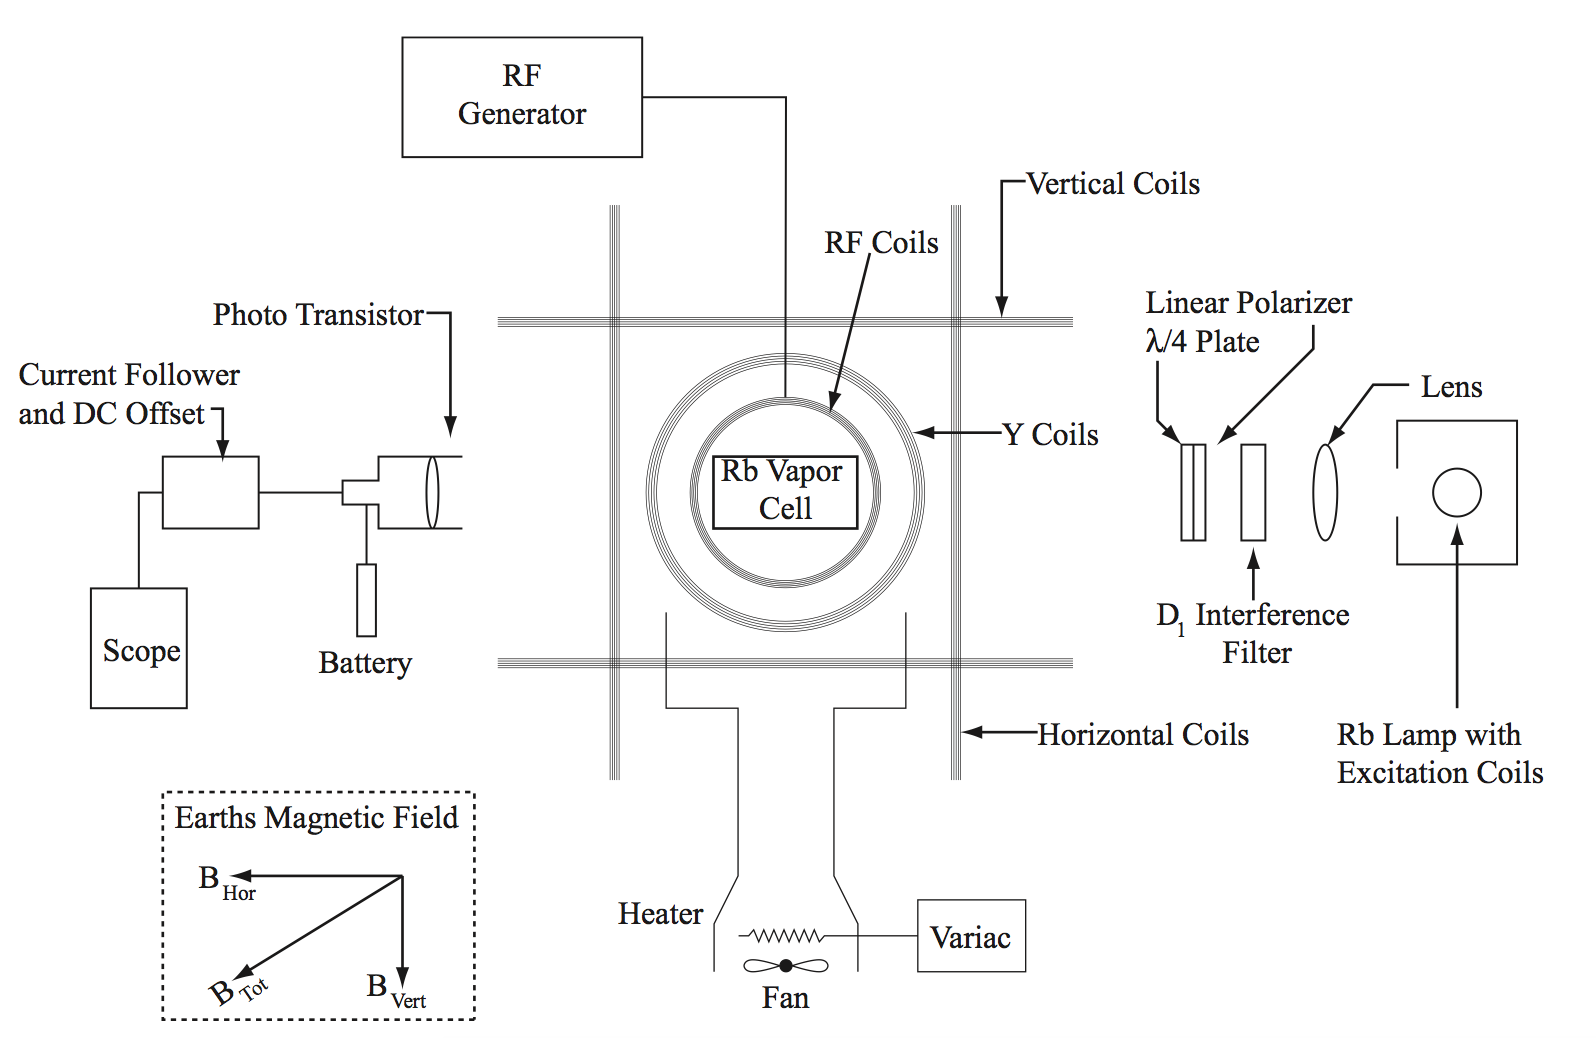
\includegraphics[scale=.05]{apparatus.png}
    \caption{Individual components are labeled, and will be discussed further subsequently.  It should be noted that the Z coils are on top of (share an axis with) the Horizontal coils in the diagram.}
  \end{figure}




\section{Data/Uncertainty Analysis}%%%%%%%%%%%%%%%%%%%%%%%%%%%%%%%%%%%%%%%%%%%%

\section{Conclusion}%%%%%%%%%%%%%%%%%%%%%%%%%%%%%%%%%%%%%%%%%%%%%%%%%%%%%%%%%%%

% \begin{thebibliography}
%
%
% \end{thebibliography}

\end{document}
